\subsection{Leaky bucket counter}


\subsubsection*{Problem}


Wie kann ein System wissen, ob ein Error transient oder sporadisch auftritt? Auch nicht-dauerhafte Fehler können zu Failures führen, sind aber ihrer transienten Natur entsprechend schwierig bis gar nicht zu isolieren und korrigieren.

Oft greift man bis zu einer bestimmten Anzahl selten auftretender Fehler gar nicht ein. Treten sie aber gehäuft ein, so soll das System eine gewisse Fehlerbearbeitung auslösen.

\subsubsection*{Lösung}


Jede zu überwachende UNIT OF MITIGATION bekommt einen LEAKY BUCKET COUNTER. Tritt ein, als transient betrachteter, Fehler auf, wird der Counter inkrementiert. Periodisch wird er aber auch dekrementiert, allerdings nie unter den Anfangswert. Erreicht der Counter nun einen vorgegebenen Threshold, wird der Fehler nicht mehr als transient, sondern als permanent betrachtet.

Die Rate, mit welcher der Bucket geleert wird, muss sorgfältig gewählt werden. Geschieht es zu oft, so werden nicht-transiente Errors gar nie identifiziert.

\begin{figure}[H]
	\centering
	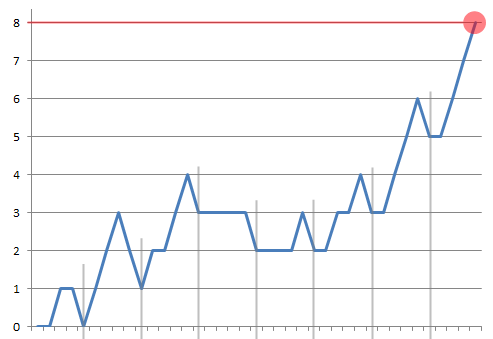
\includegraphics[width=\textwidth]{content/faulttolerance/images/leaky_bucket_counter.png}
	\caption{leaky bucket counter}
\end{figure}


